\documentclass{article}

\usepackage[margin=1in]{geometry}
\usepackage{amsmath}
\usepackage{amssymb}
\usepackage{graphicx}

\graphicspath{{./../figures/}}

\title{Assignment 2}
\author{Vignesh M Pai (20211132)}
\date{}

\begin{document}

\maketitle

\section*{1. a)}

\begin{align*}
    \int_0^1 \frac{4}{1 + x^2} dx = \input{../data/1a.dat}
\end{align*}

\section*{1. b)}

\begin{center}
    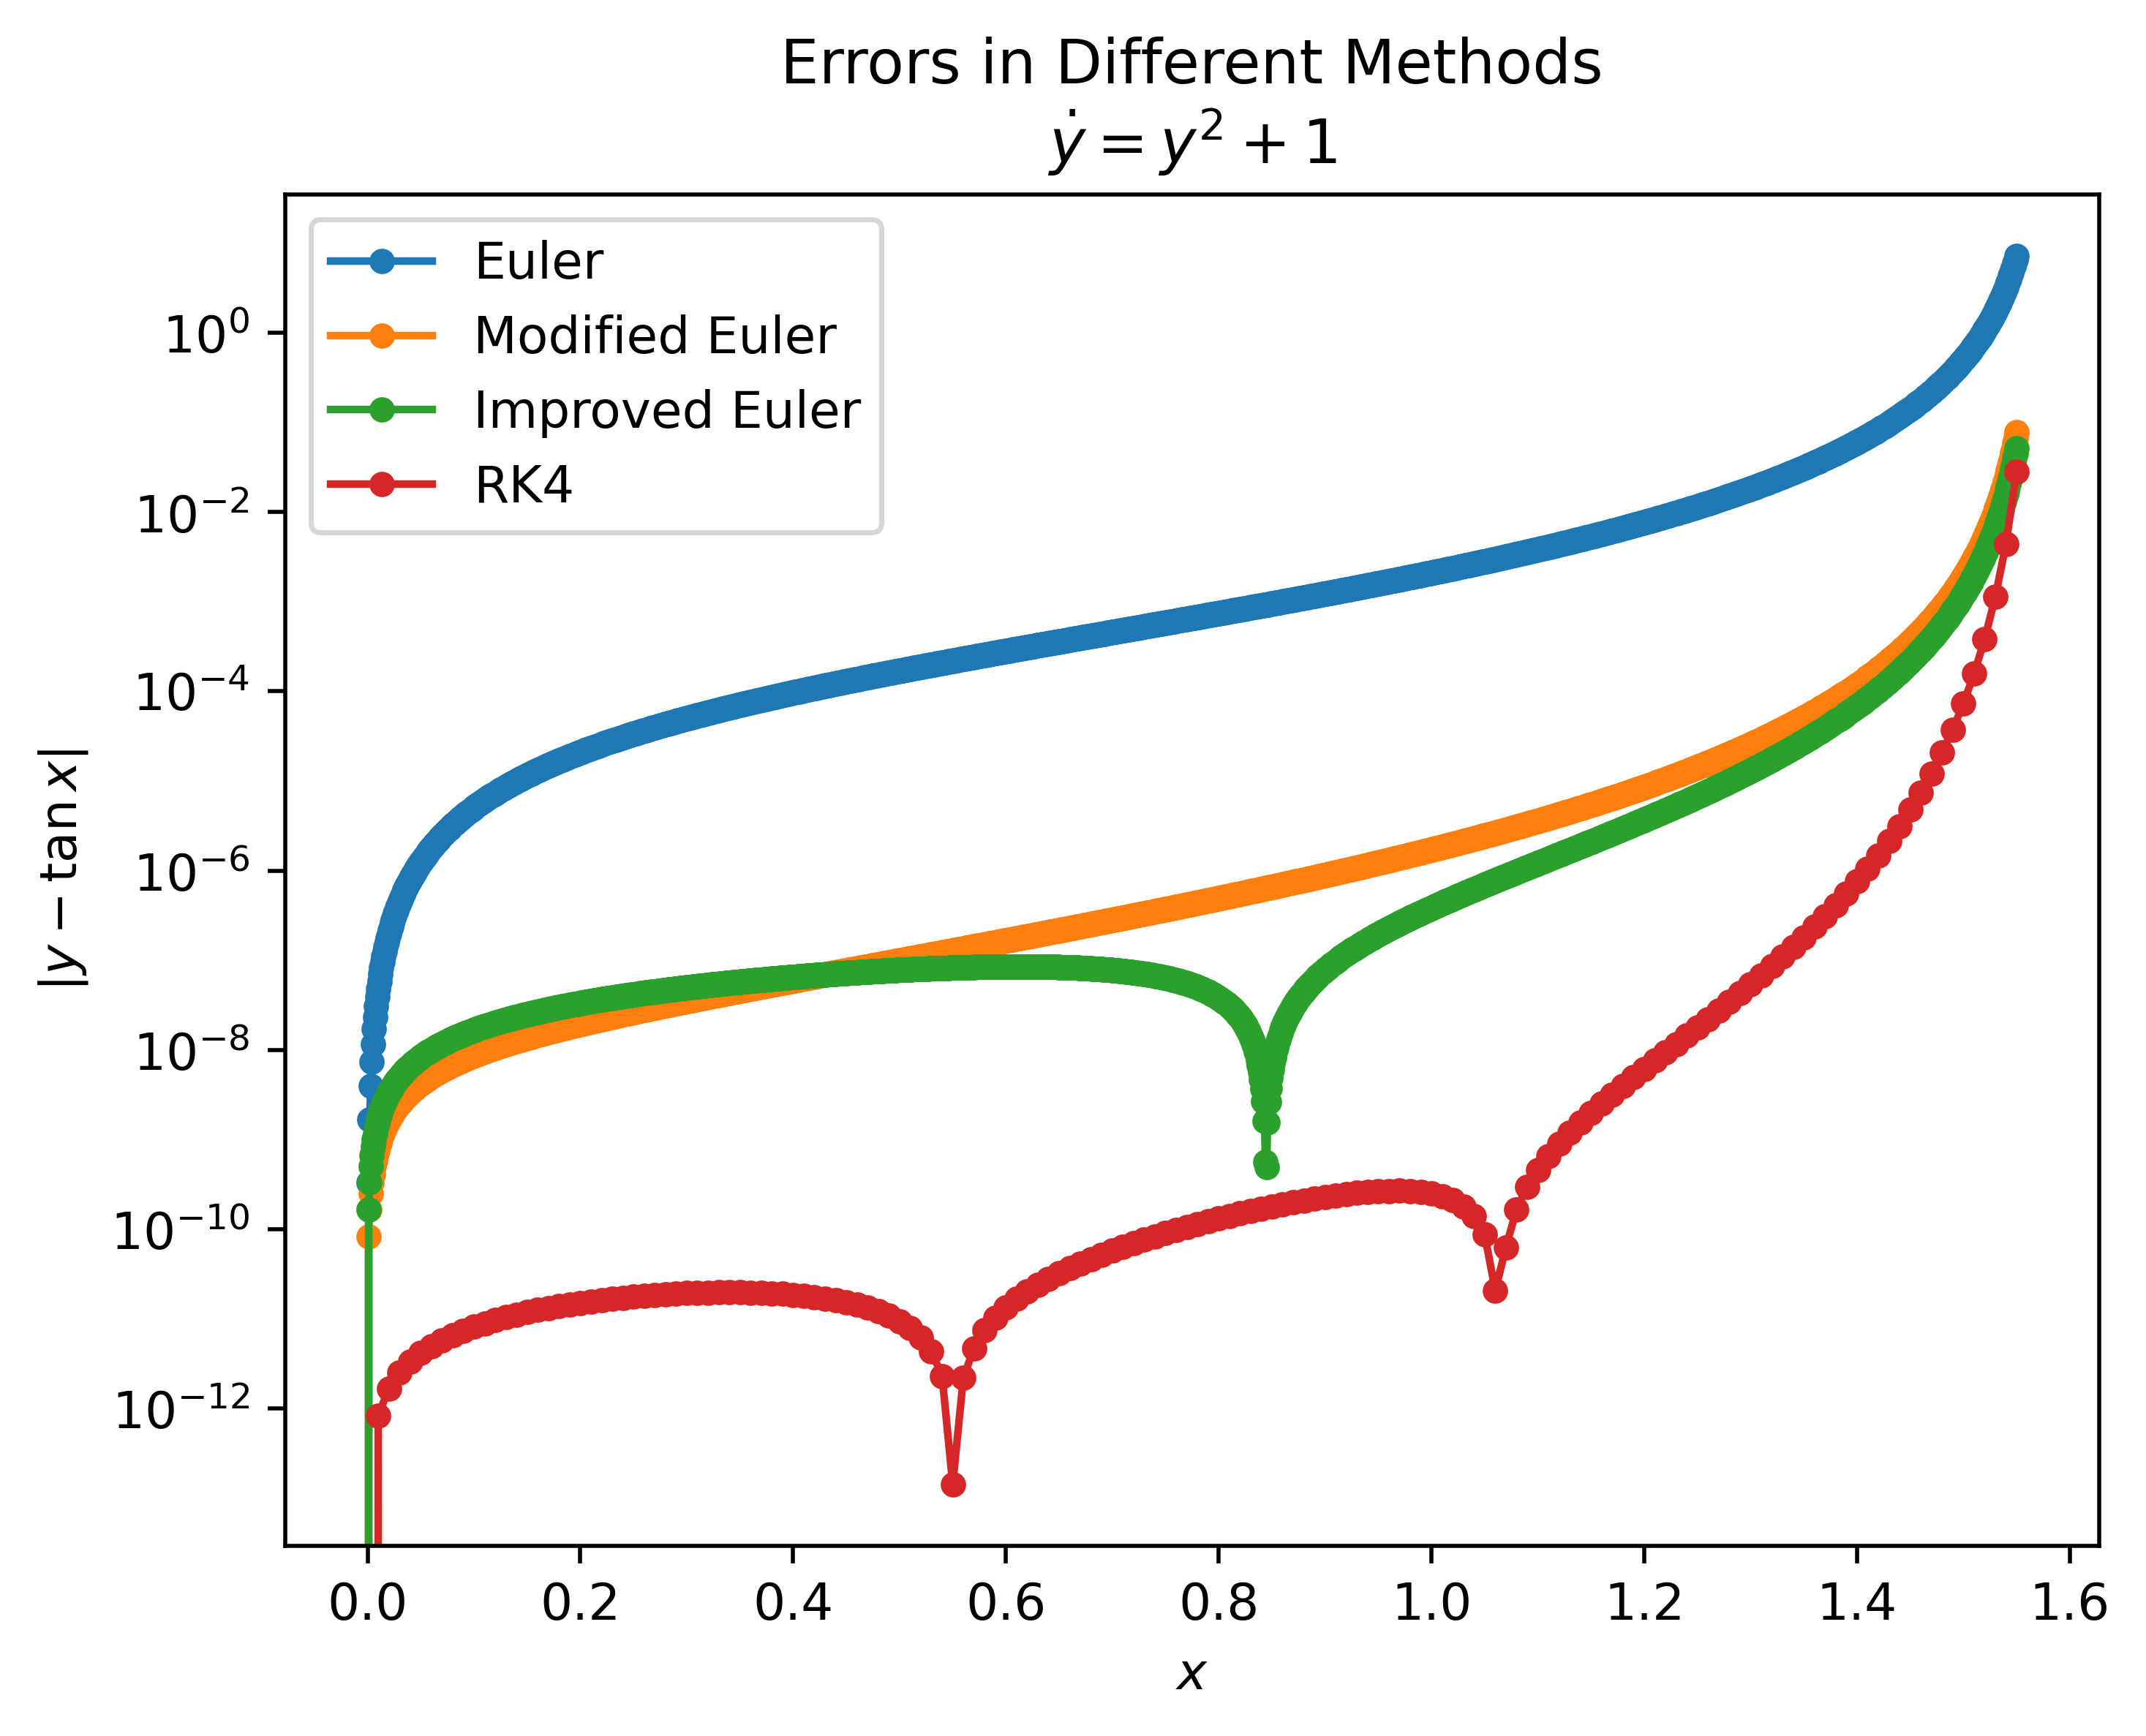
\includegraphics[scale=0.7]{1b.png}
\end{center}

\section*{1. c)}

\begin{align*}
    \int_0^\pi \sin x dx = \input{../data/1c.dat}
\end{align*}

\section*{1. d)}

\begin{align*}
    \int_0^\pi \frac{1}{2\pi} \exp\left(-\frac{x^2}{2}\right) dx = \input{../data/1d.dat}
\end{align*}

\section*{2. a)}

\begin{center}
    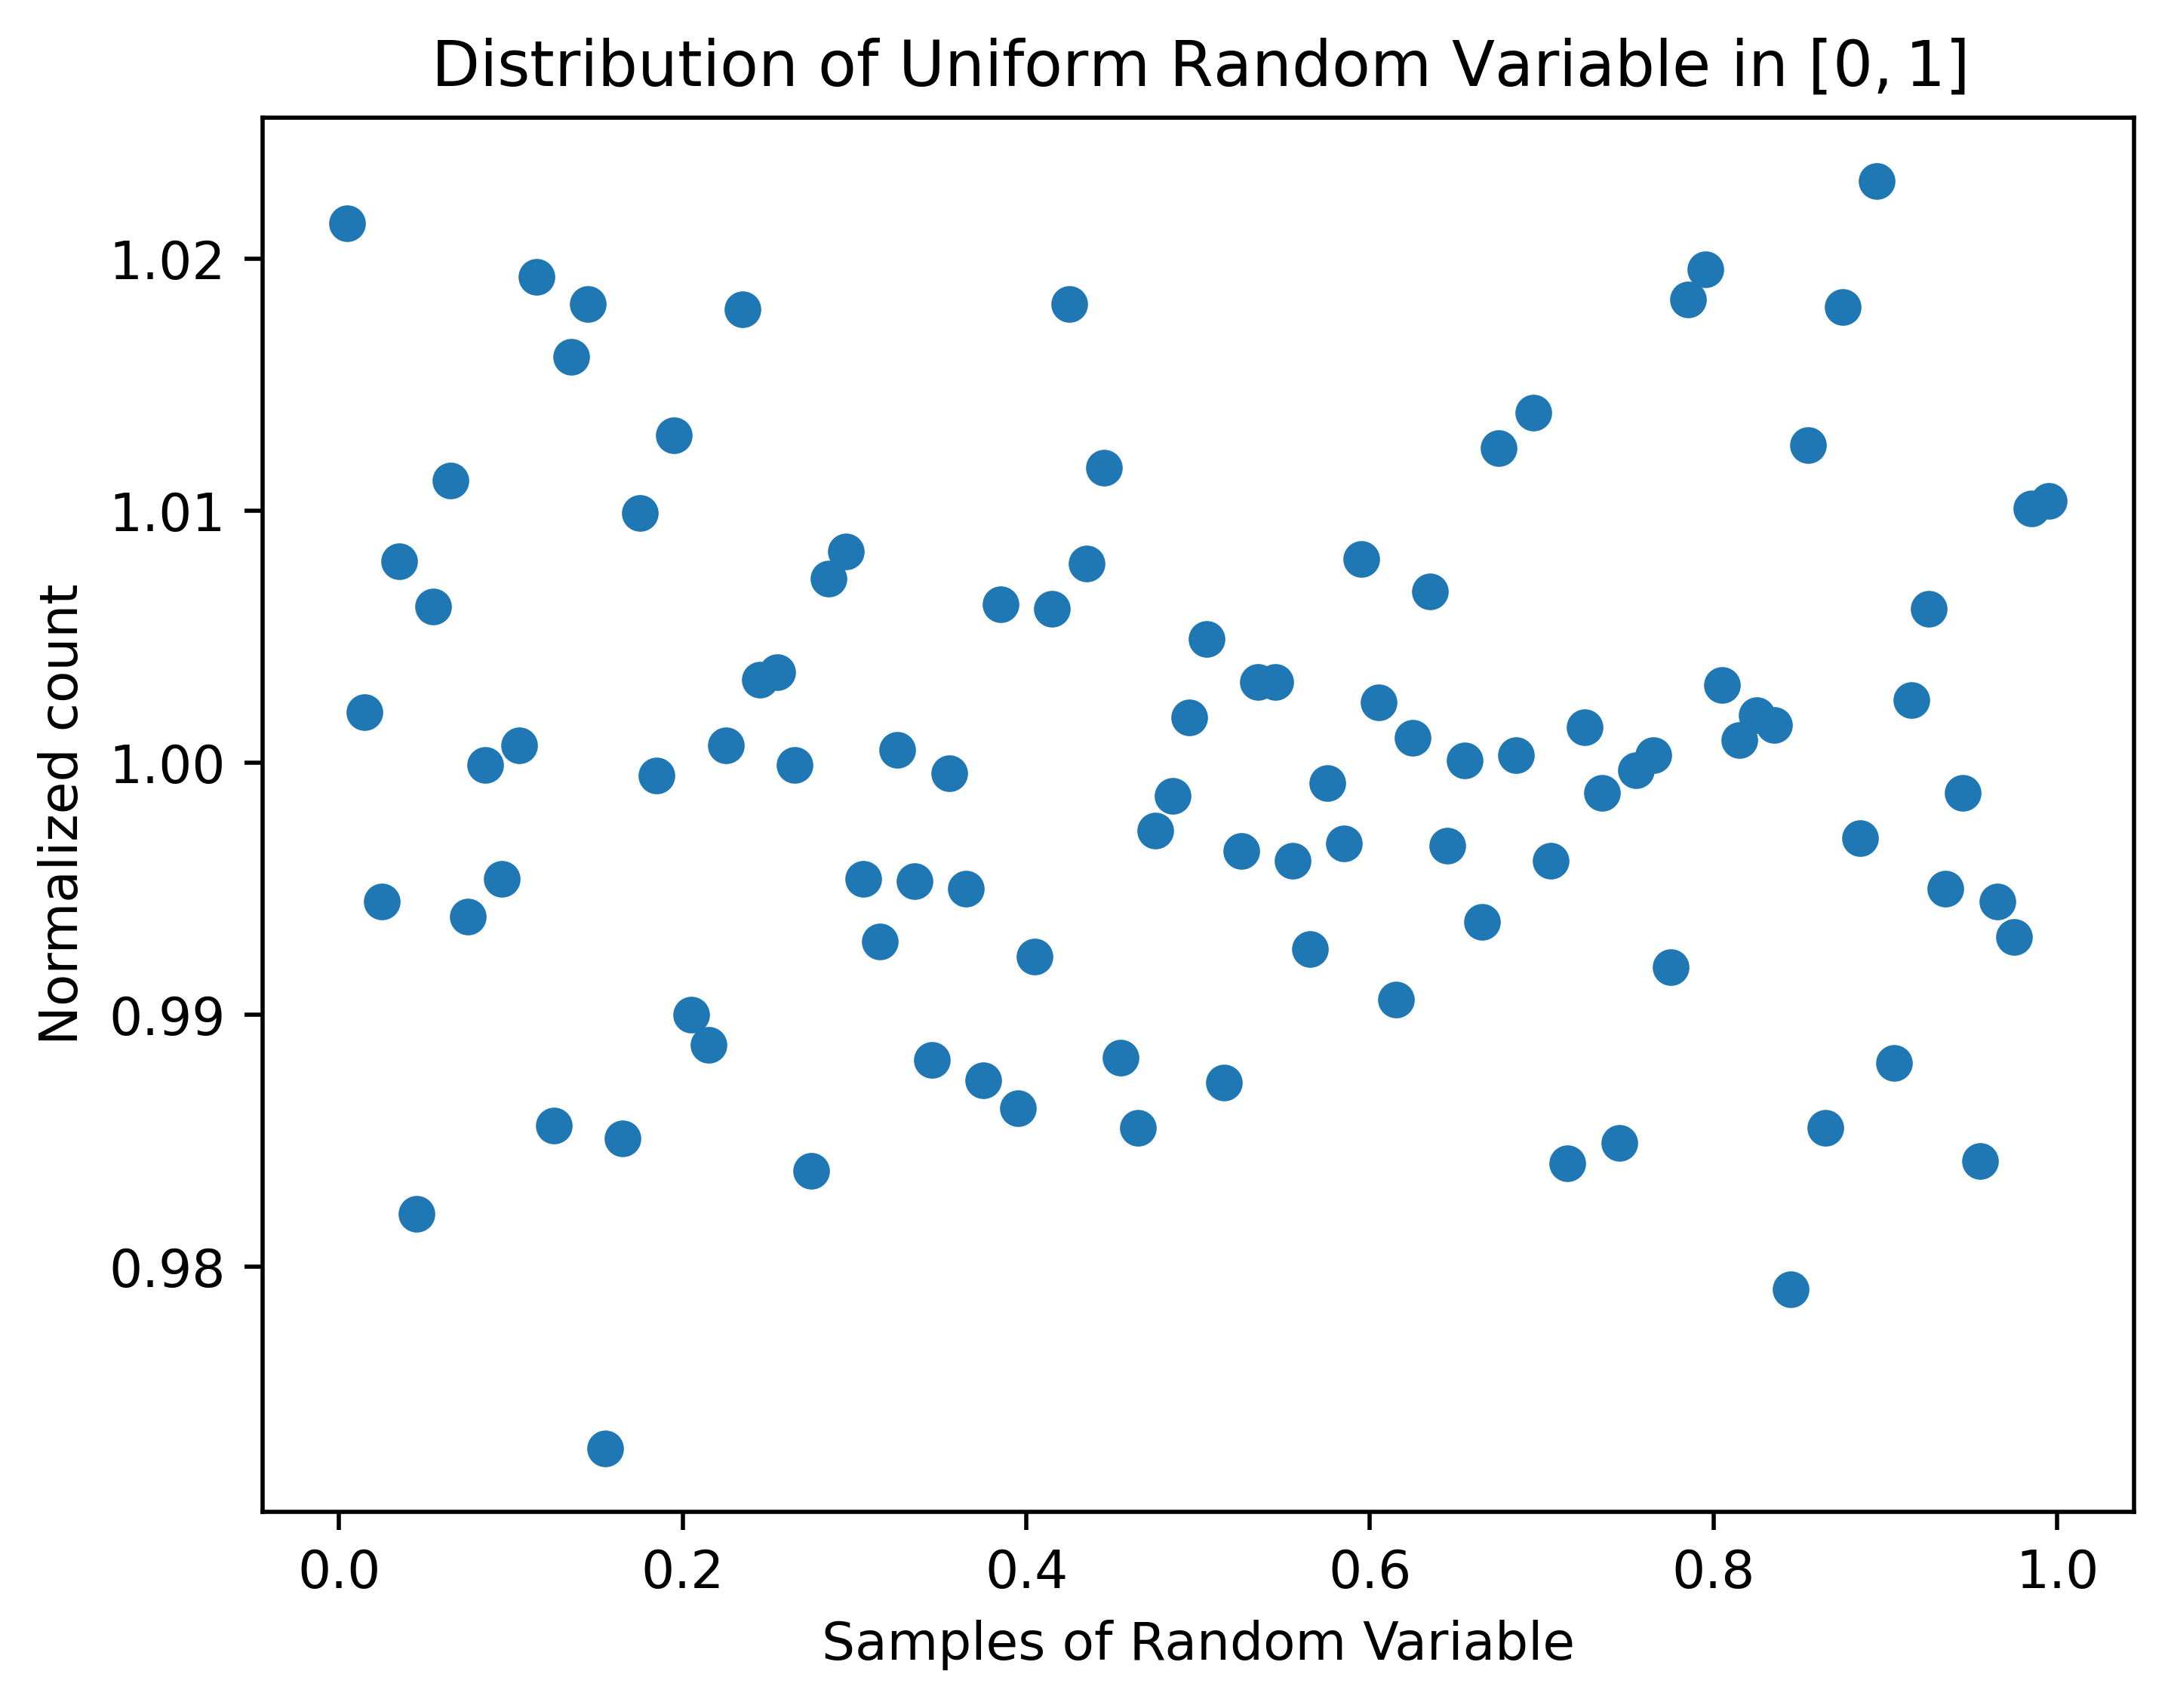
\includegraphics[scale=0.7]{2a.png}
\end{center}

\section*{2. b)}

\begin{center}
    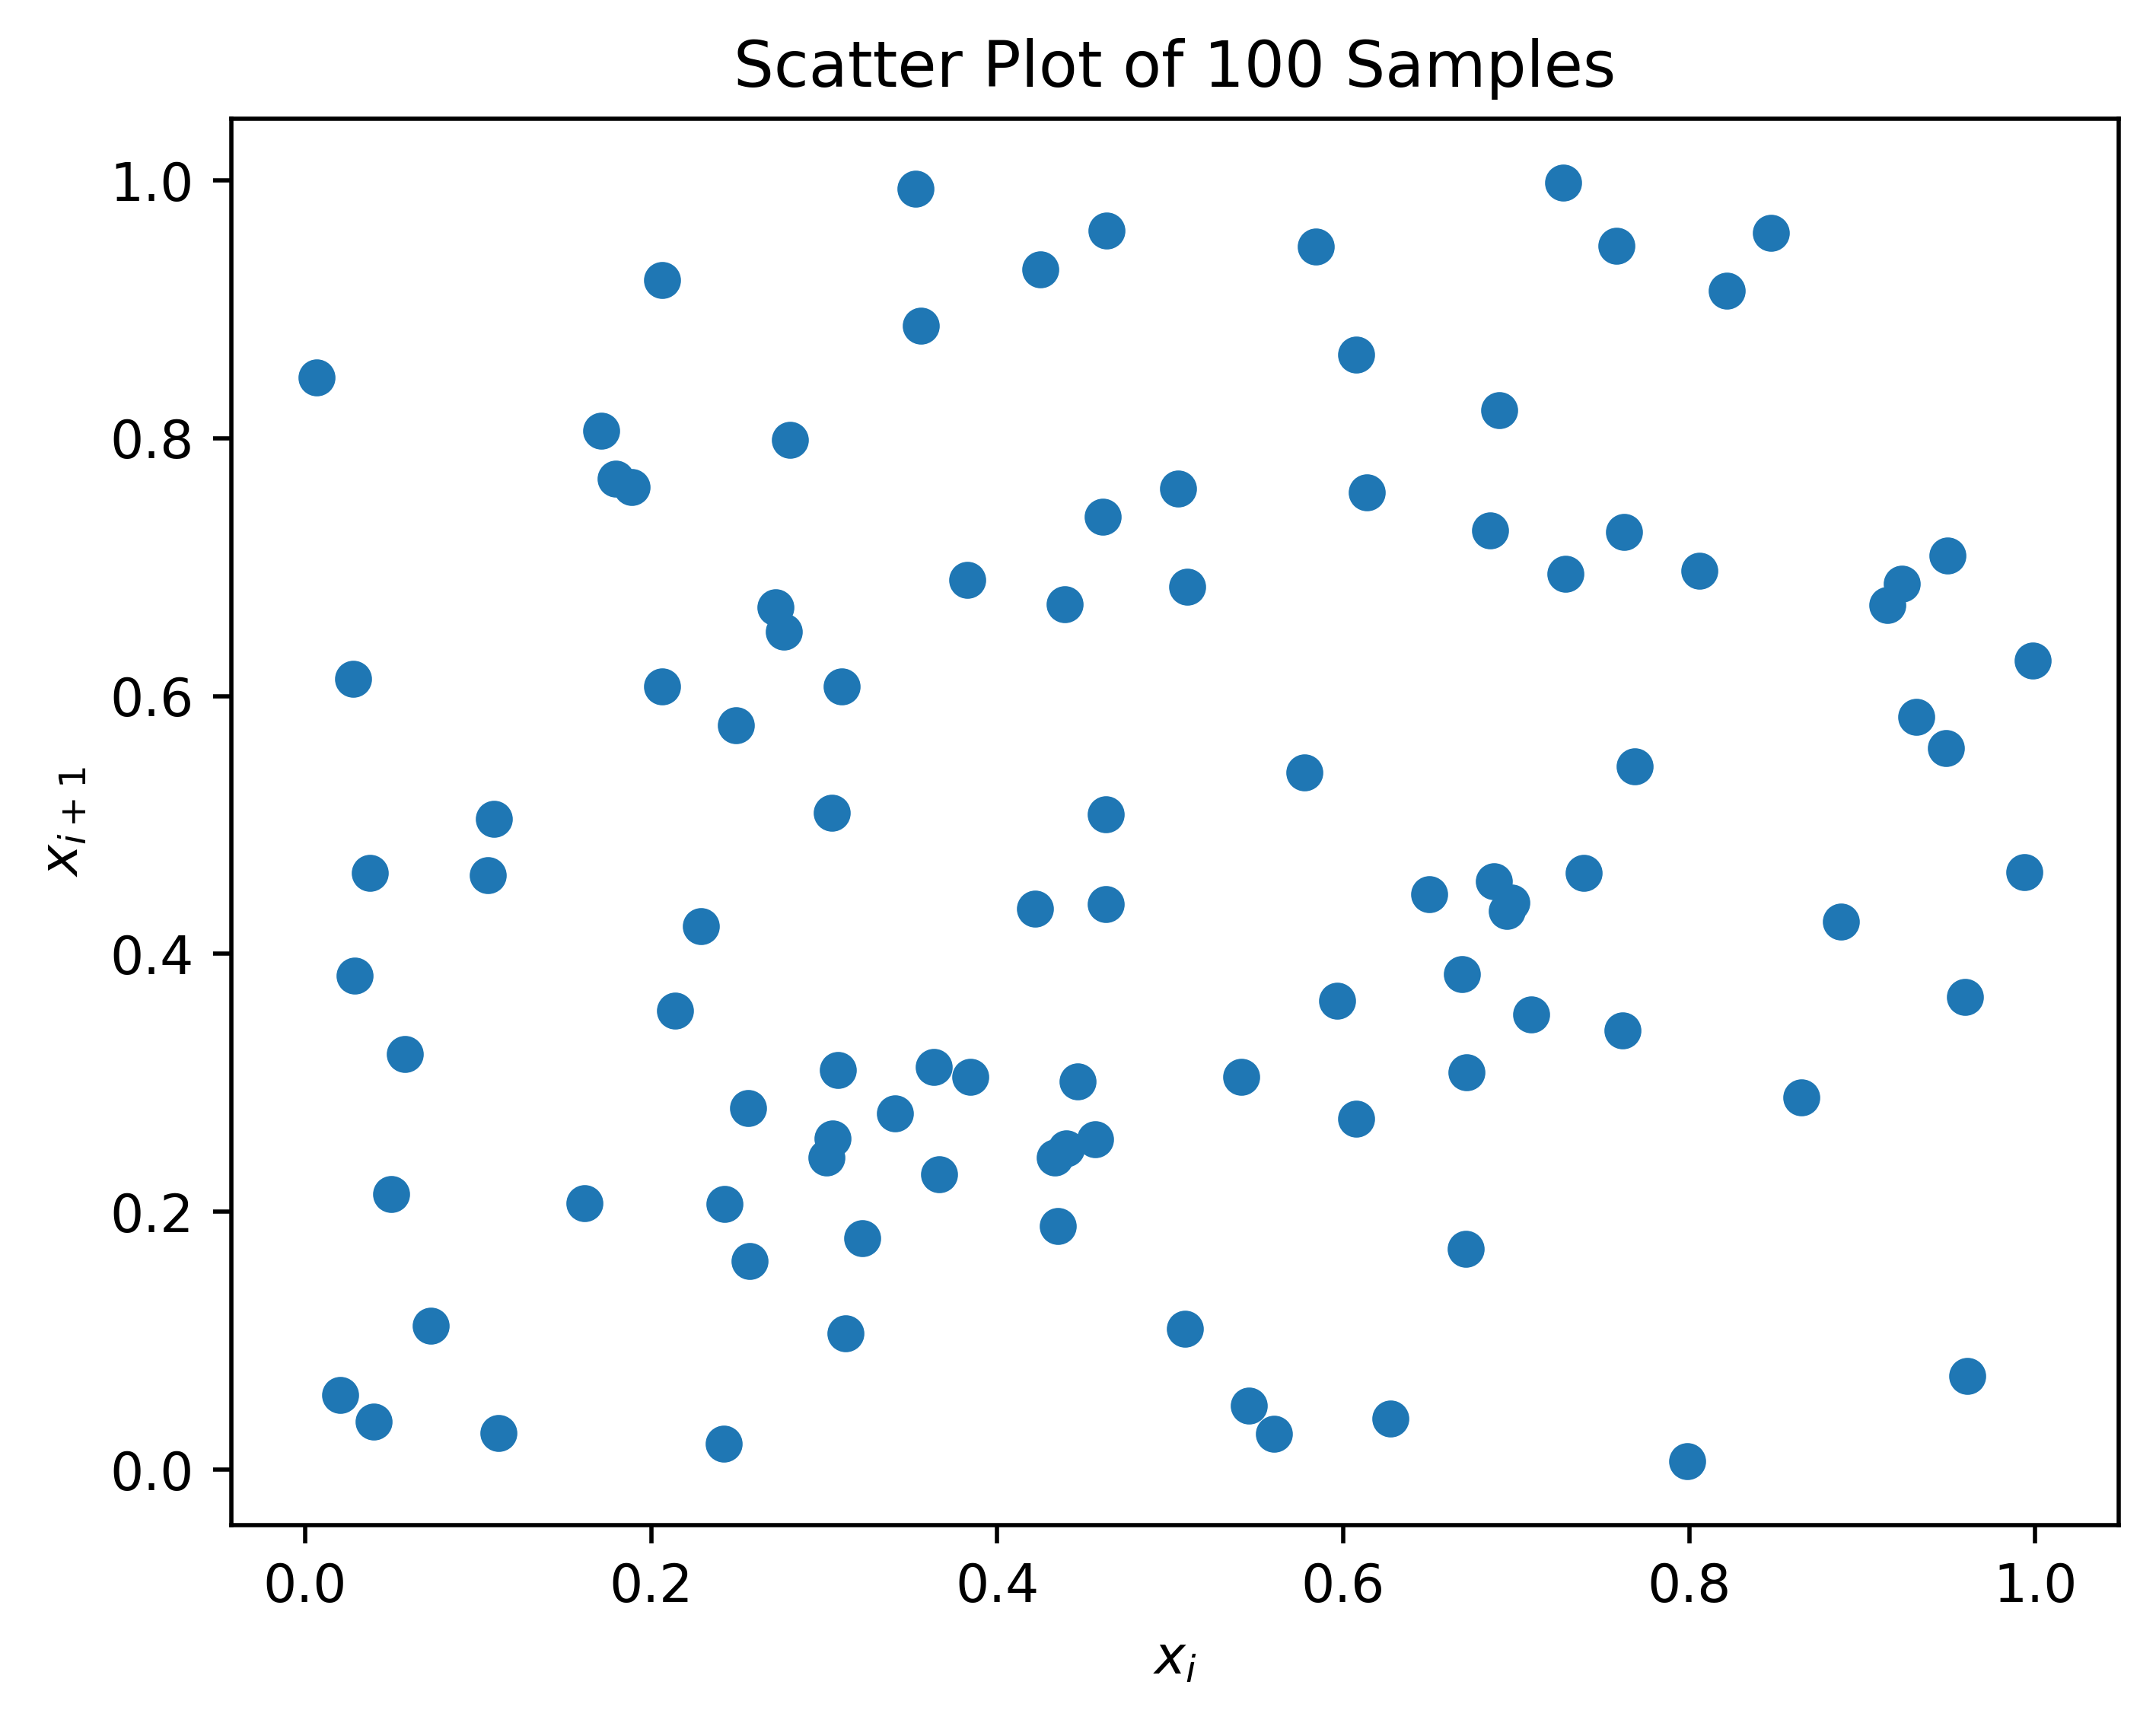
\includegraphics[scale=0.7]{2b.png}
\end{center}

\section*{2. c)}

\begin{center}
    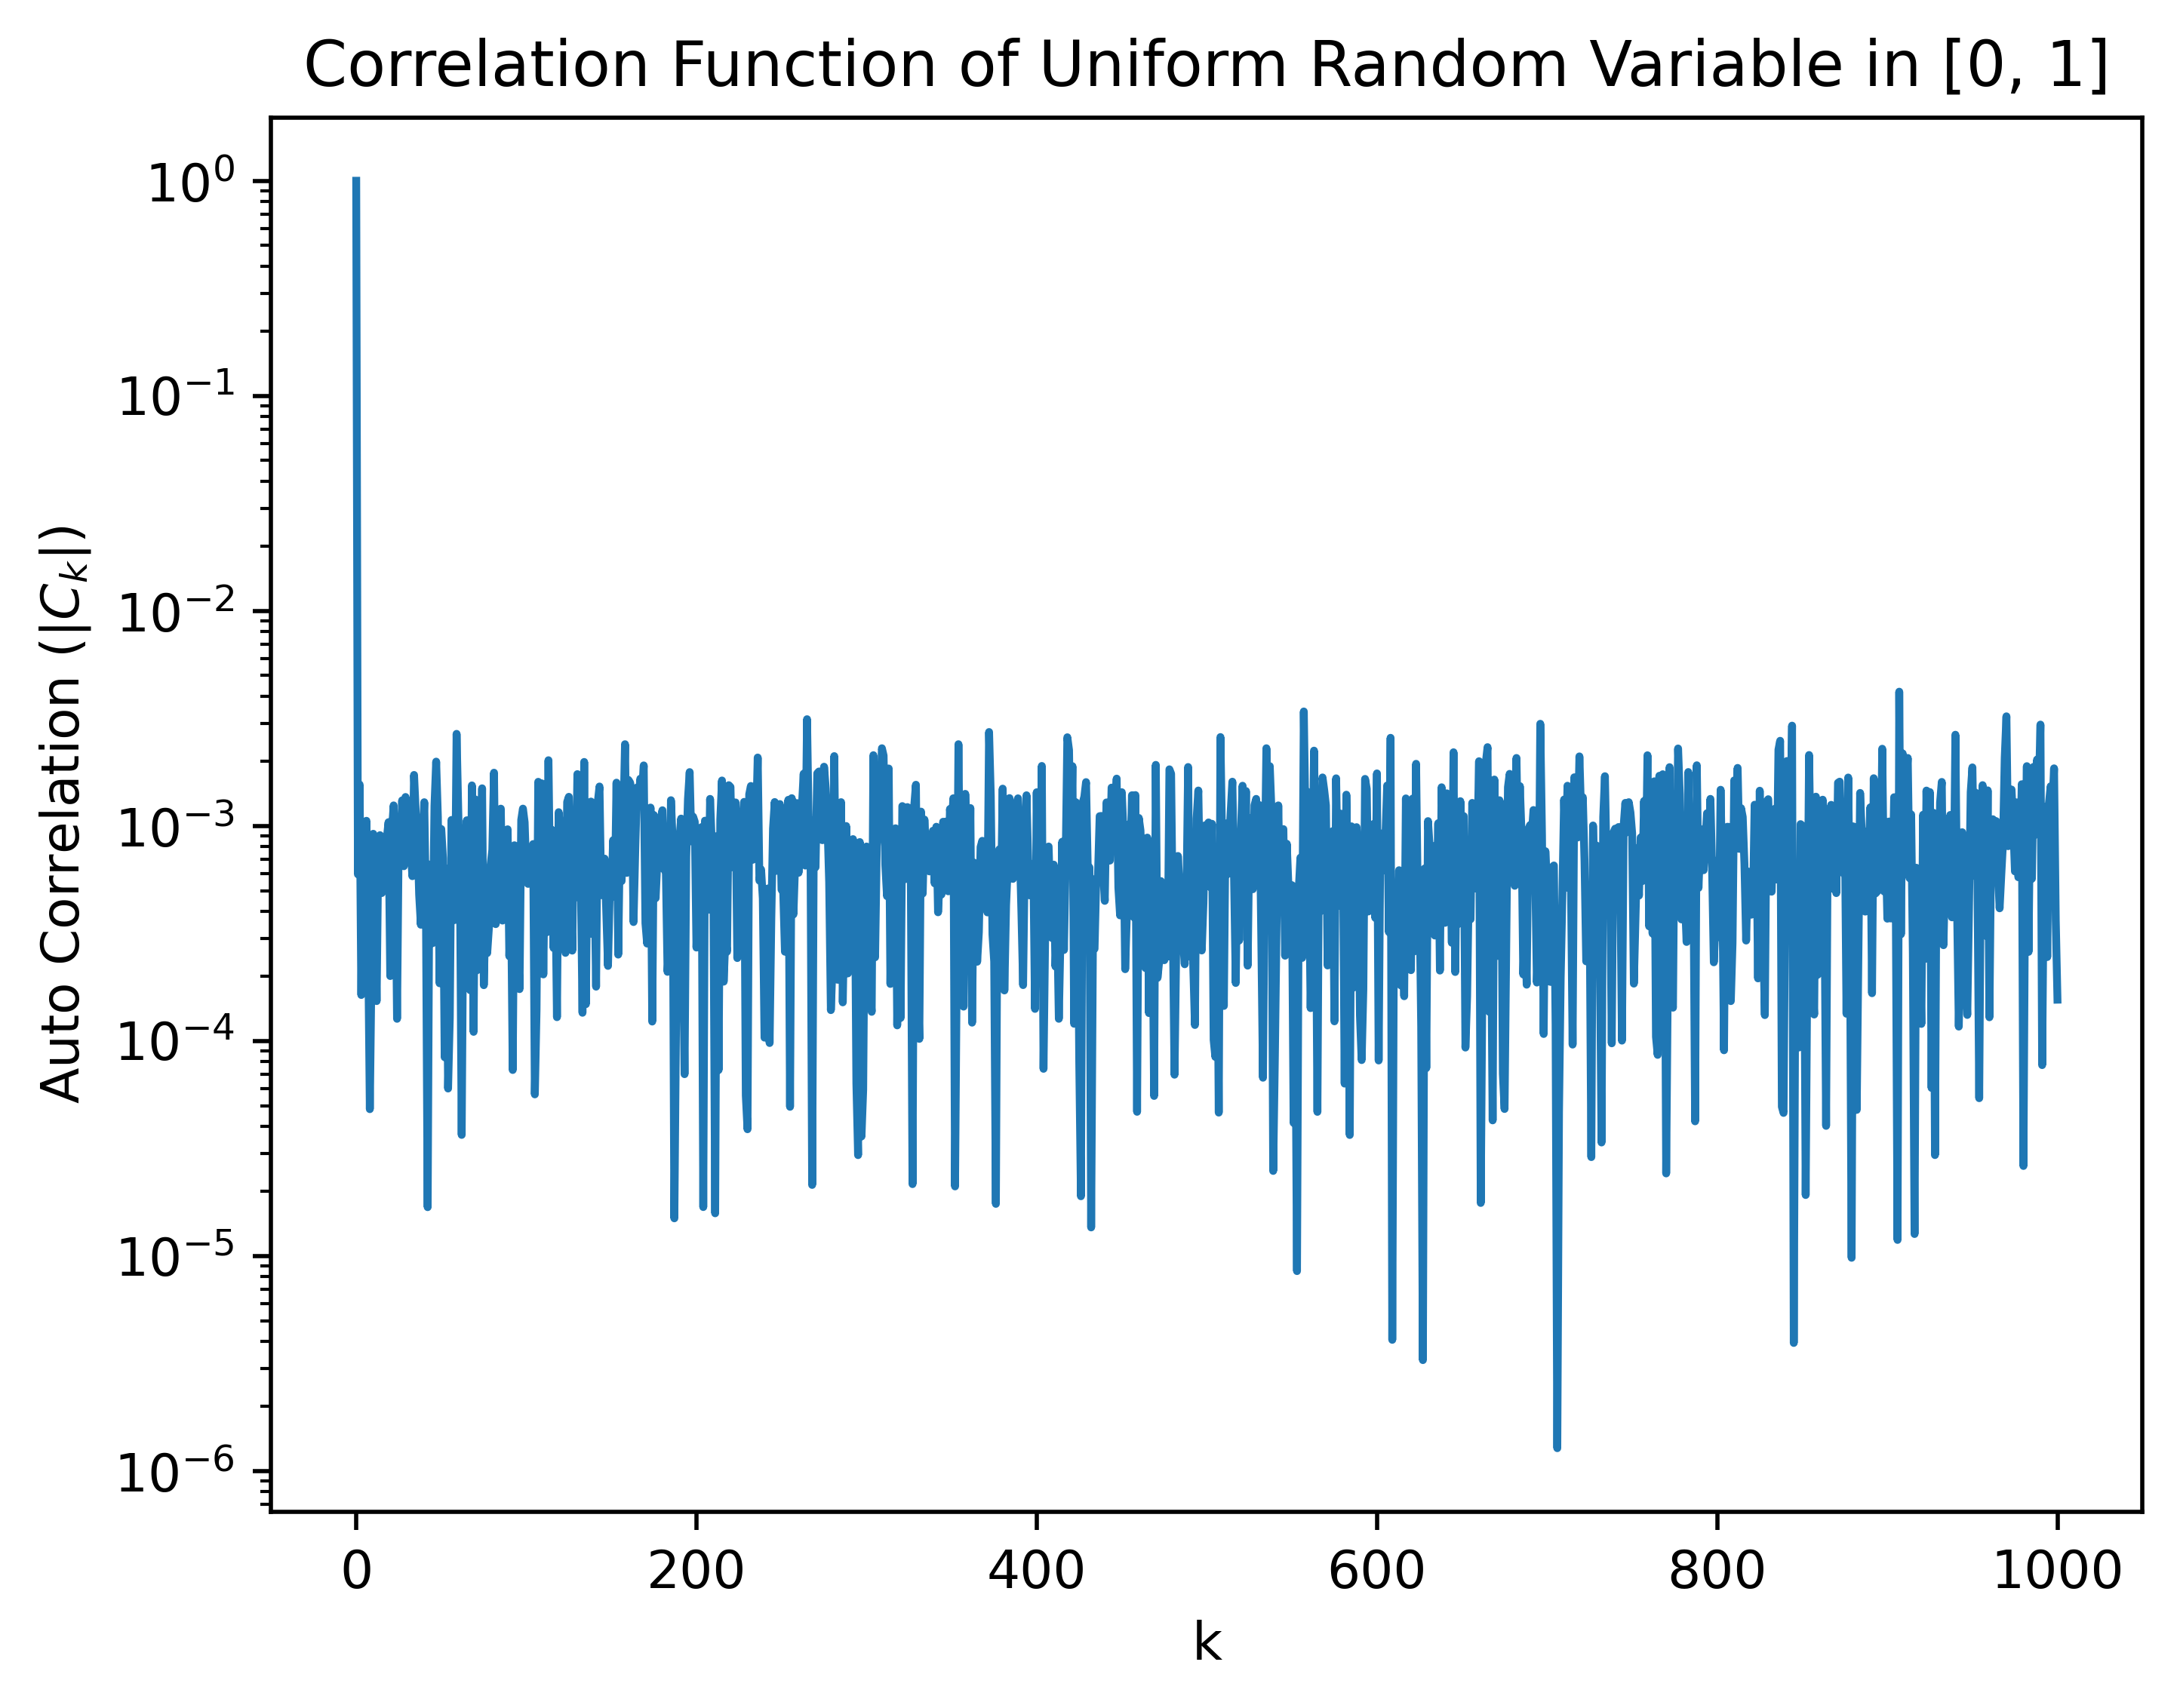
\includegraphics[scale=0.7]{2c.png}
\end{center}

\section*{2. d)}

\begin{center}
    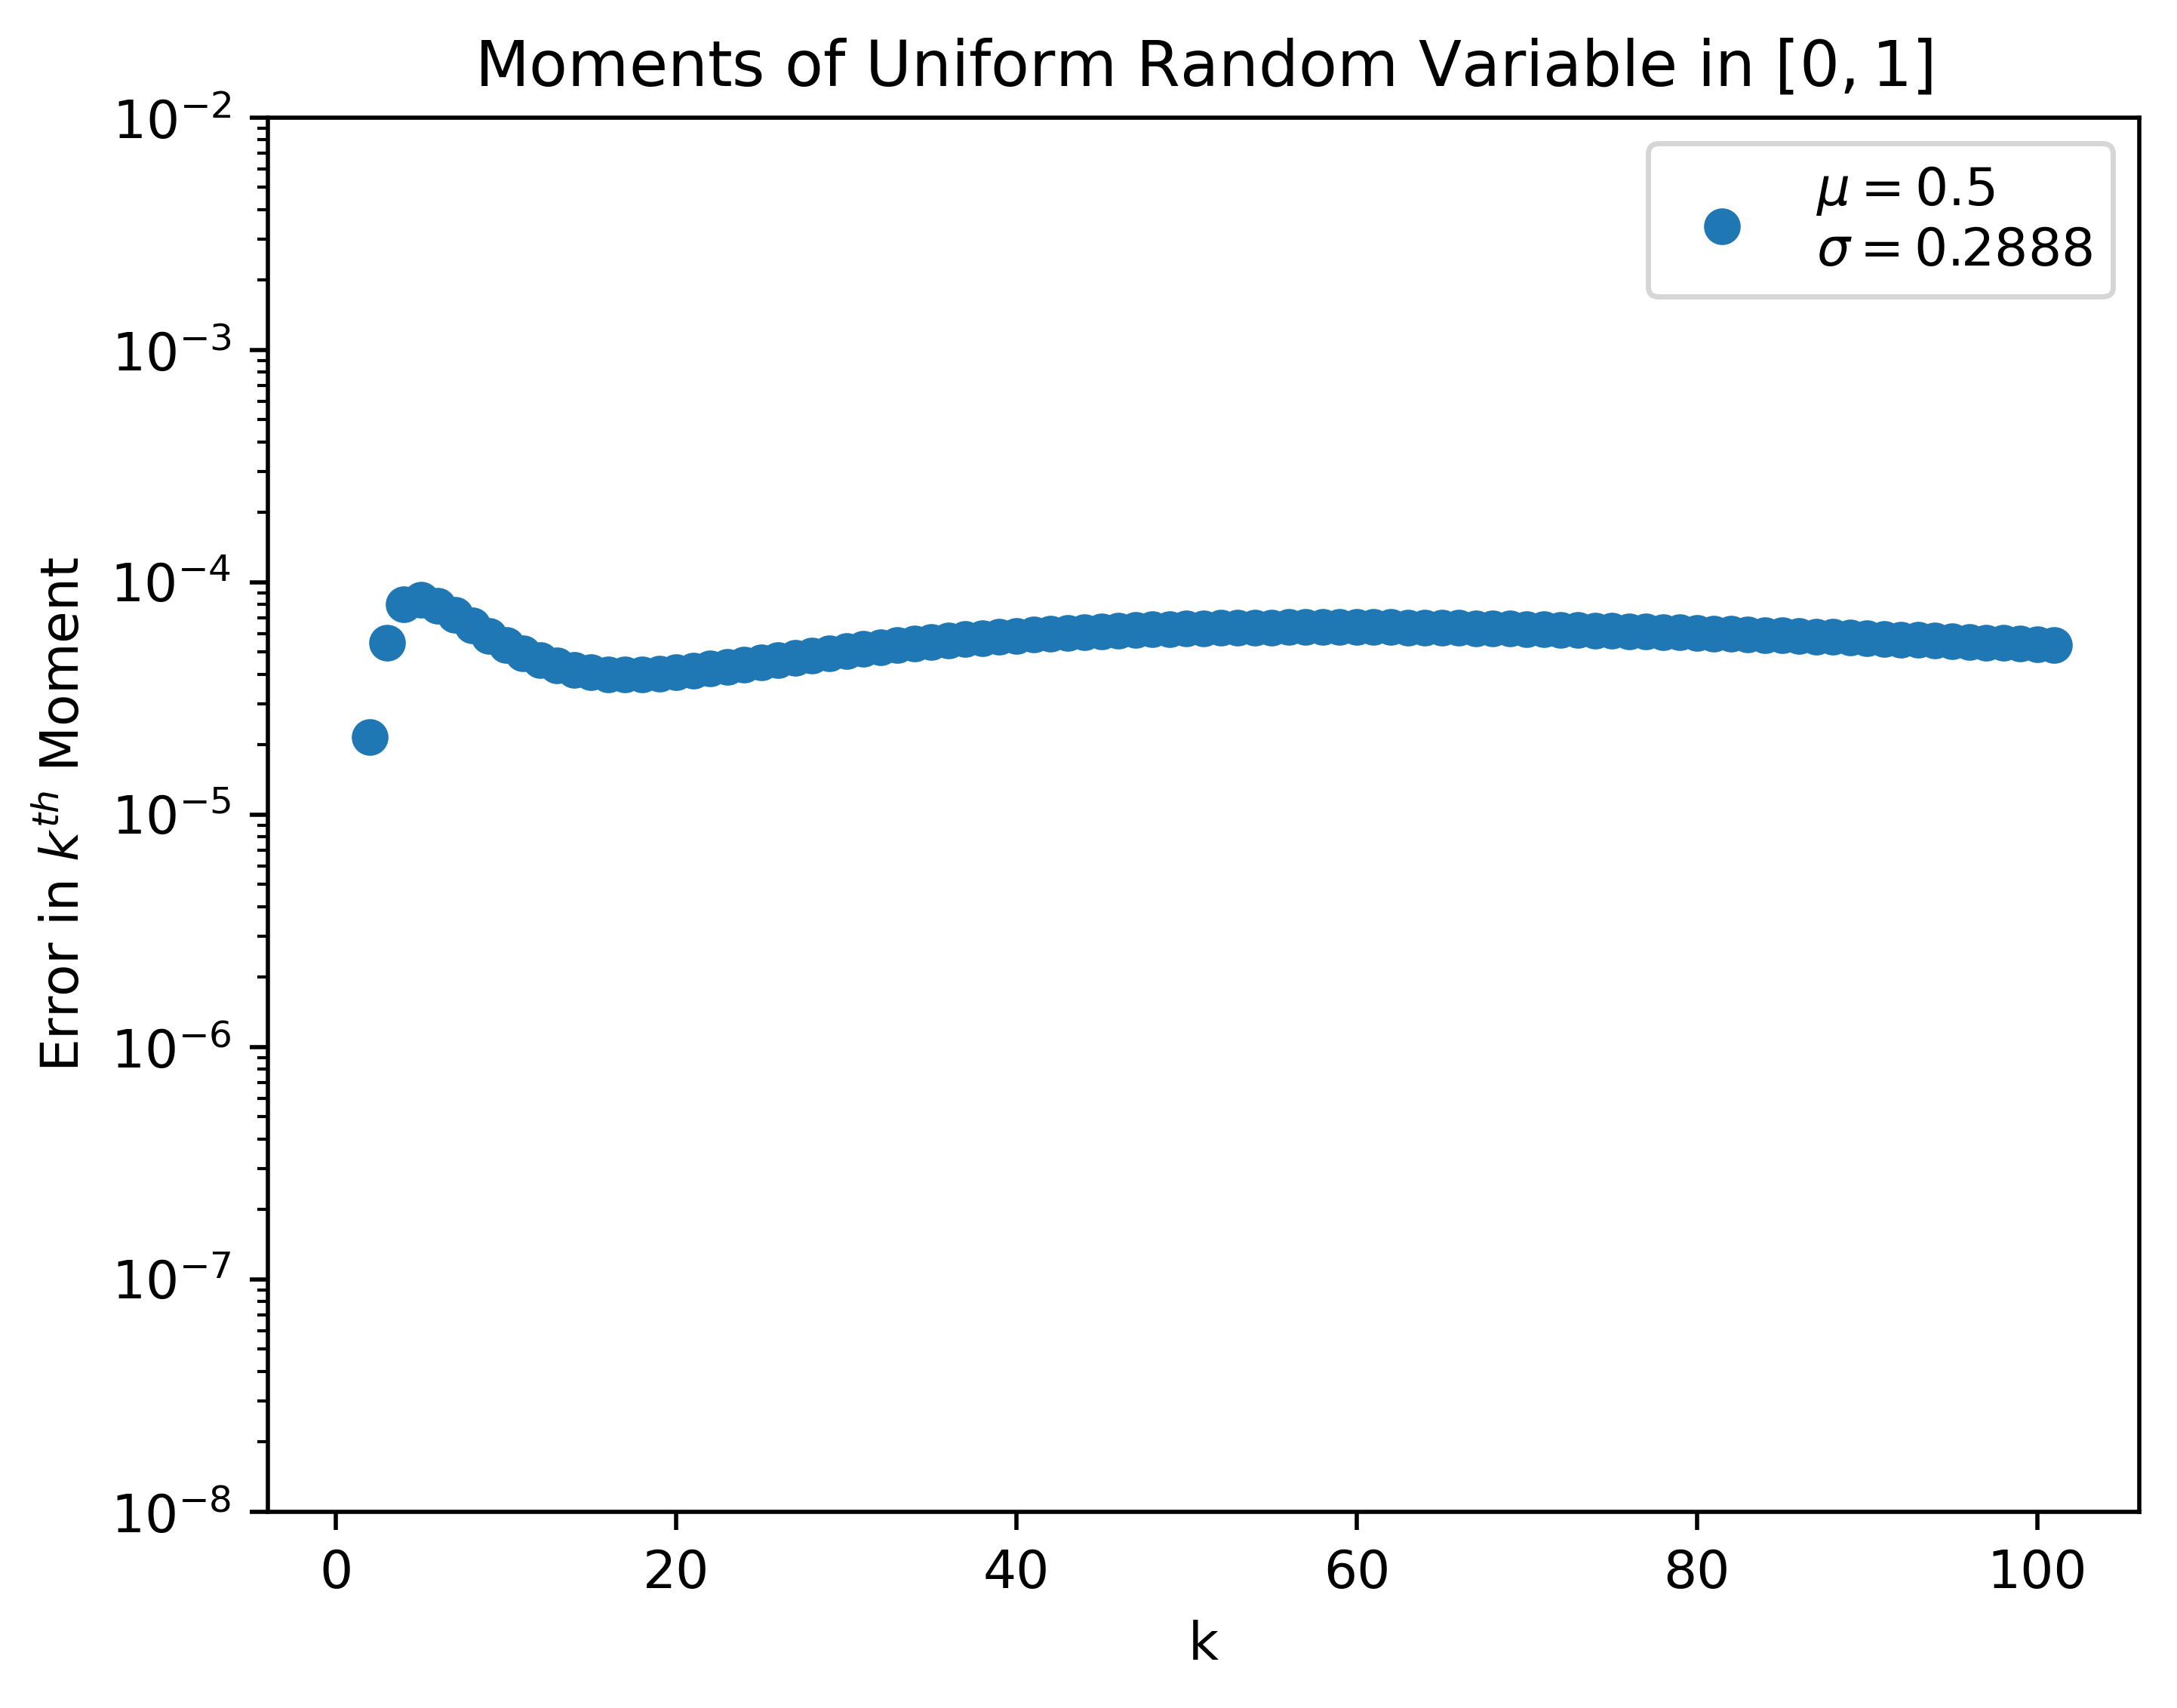
\includegraphics[scale=0.7]{2d.png}
\end{center}

\section*{4. a)}

\begin{center}
    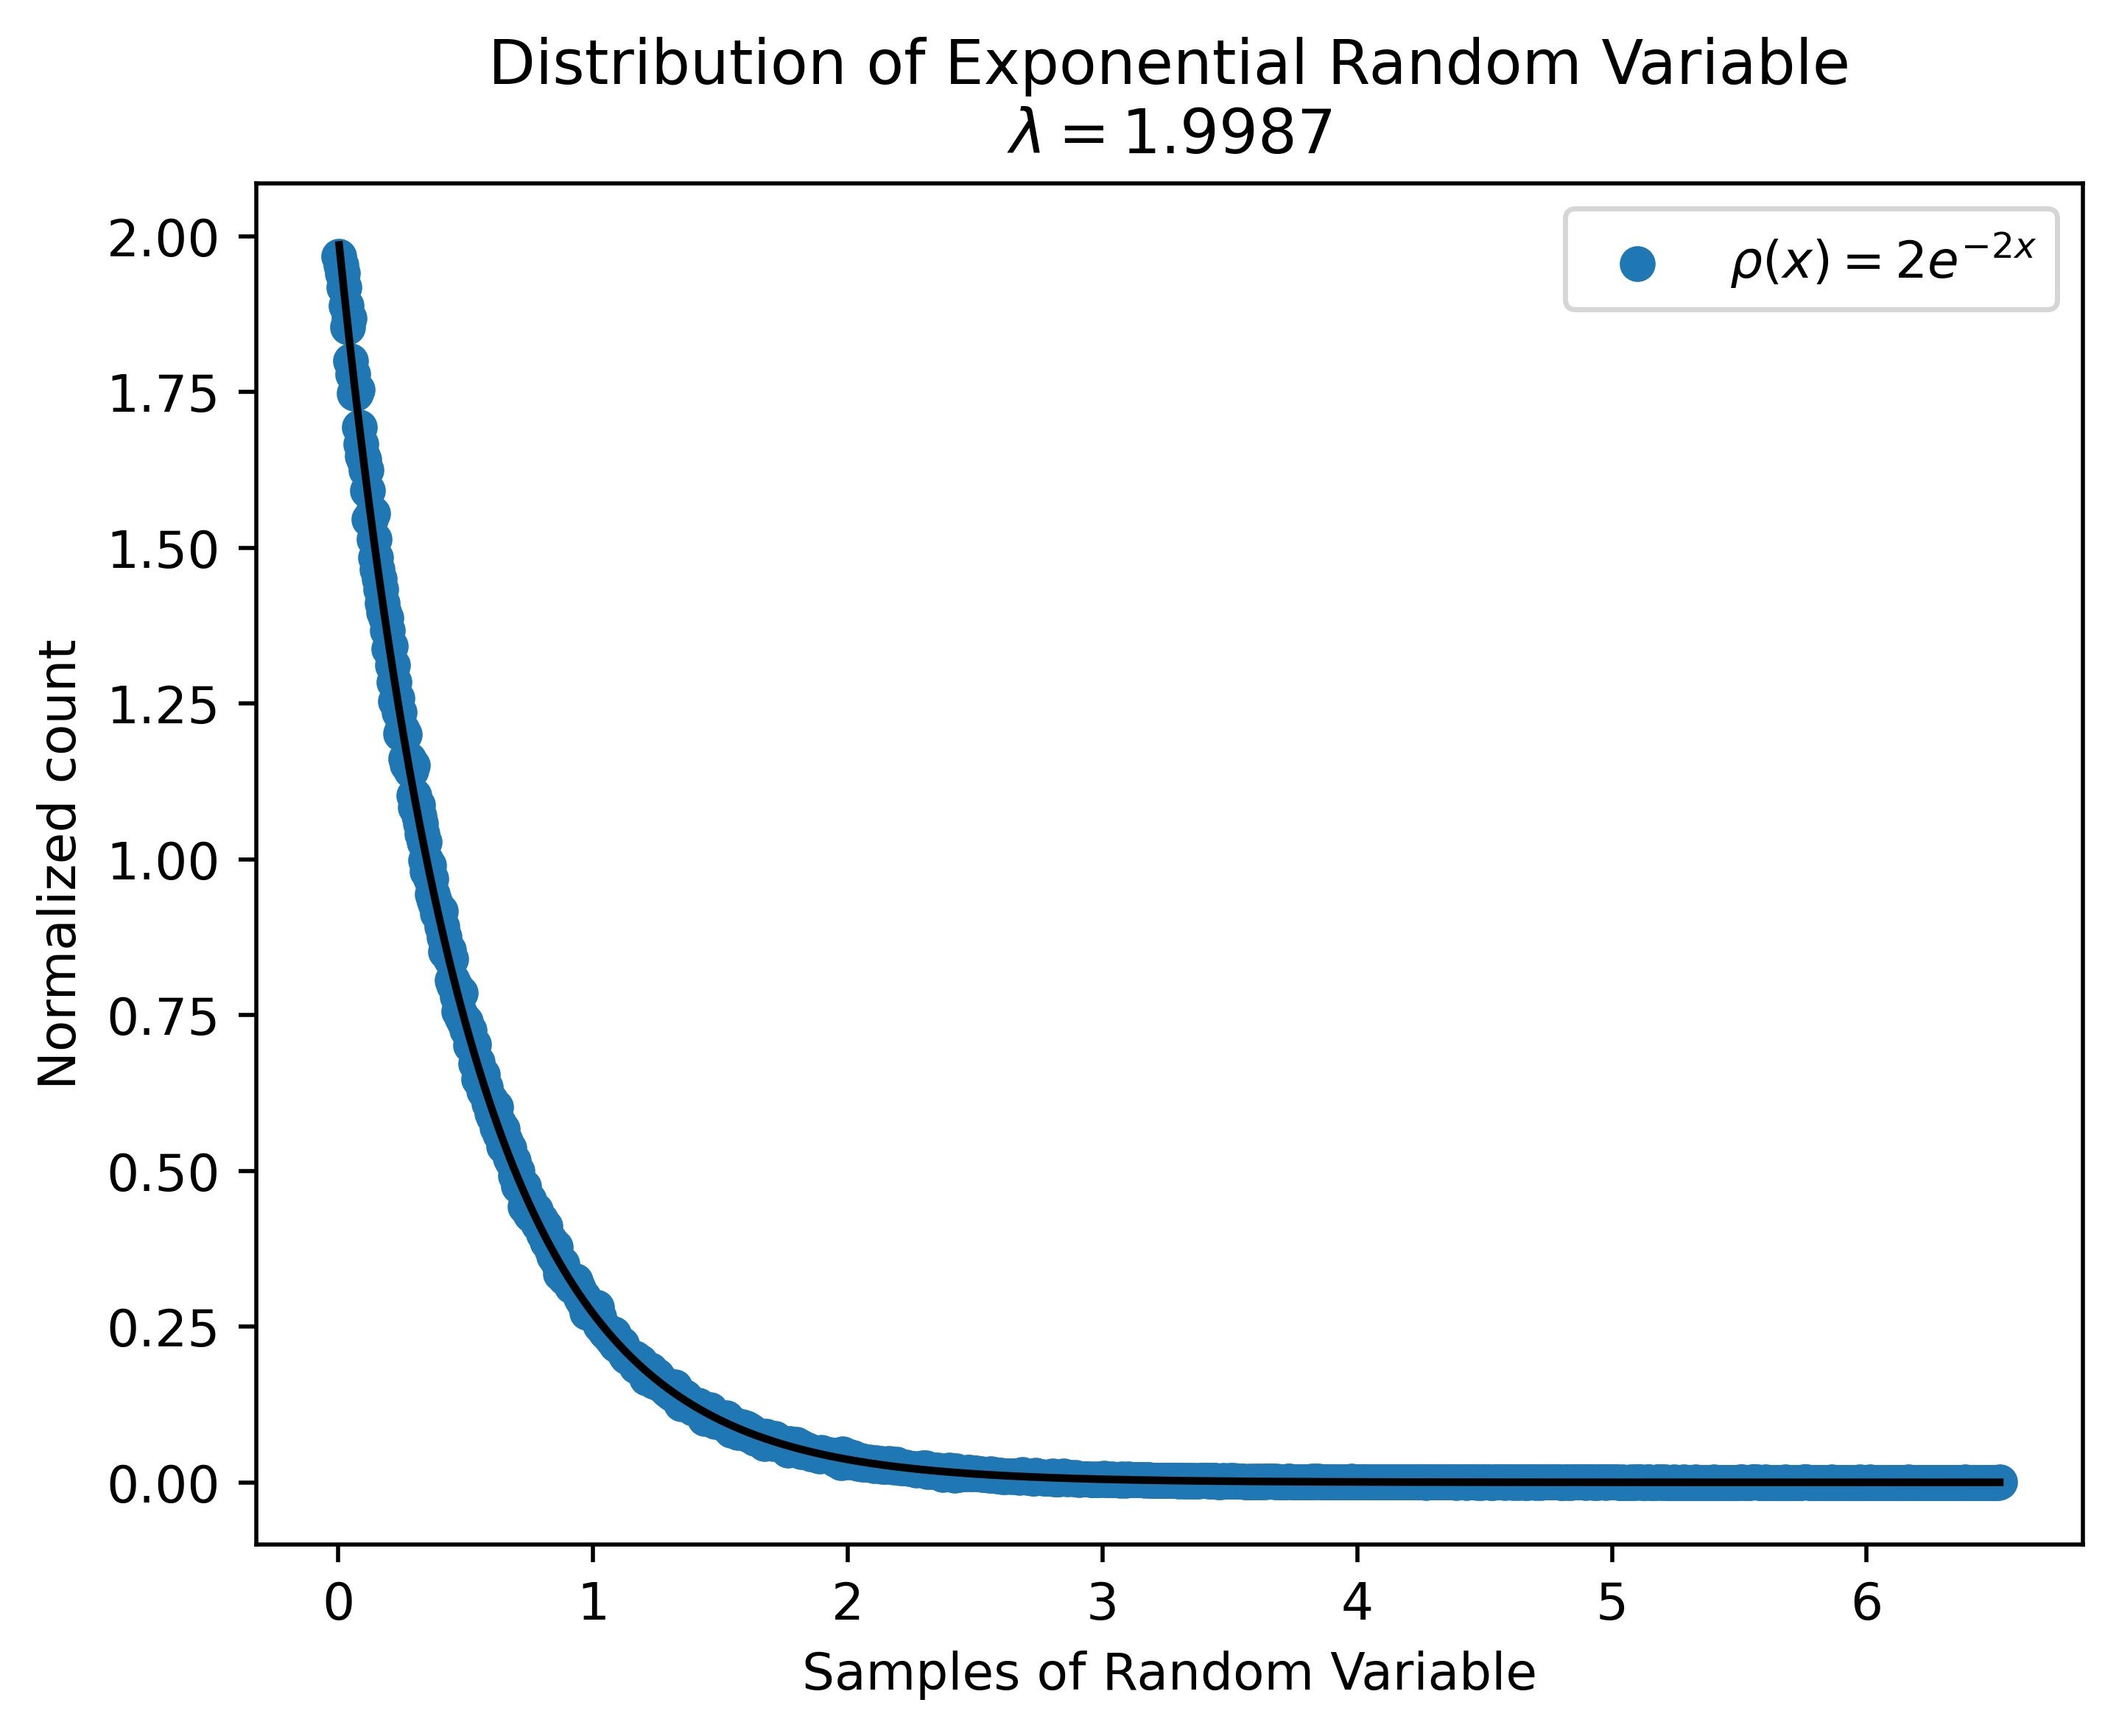
\includegraphics[scale=0.7]{4a.png}
\end{center}

\section*{4. b)}

\begin{center}
    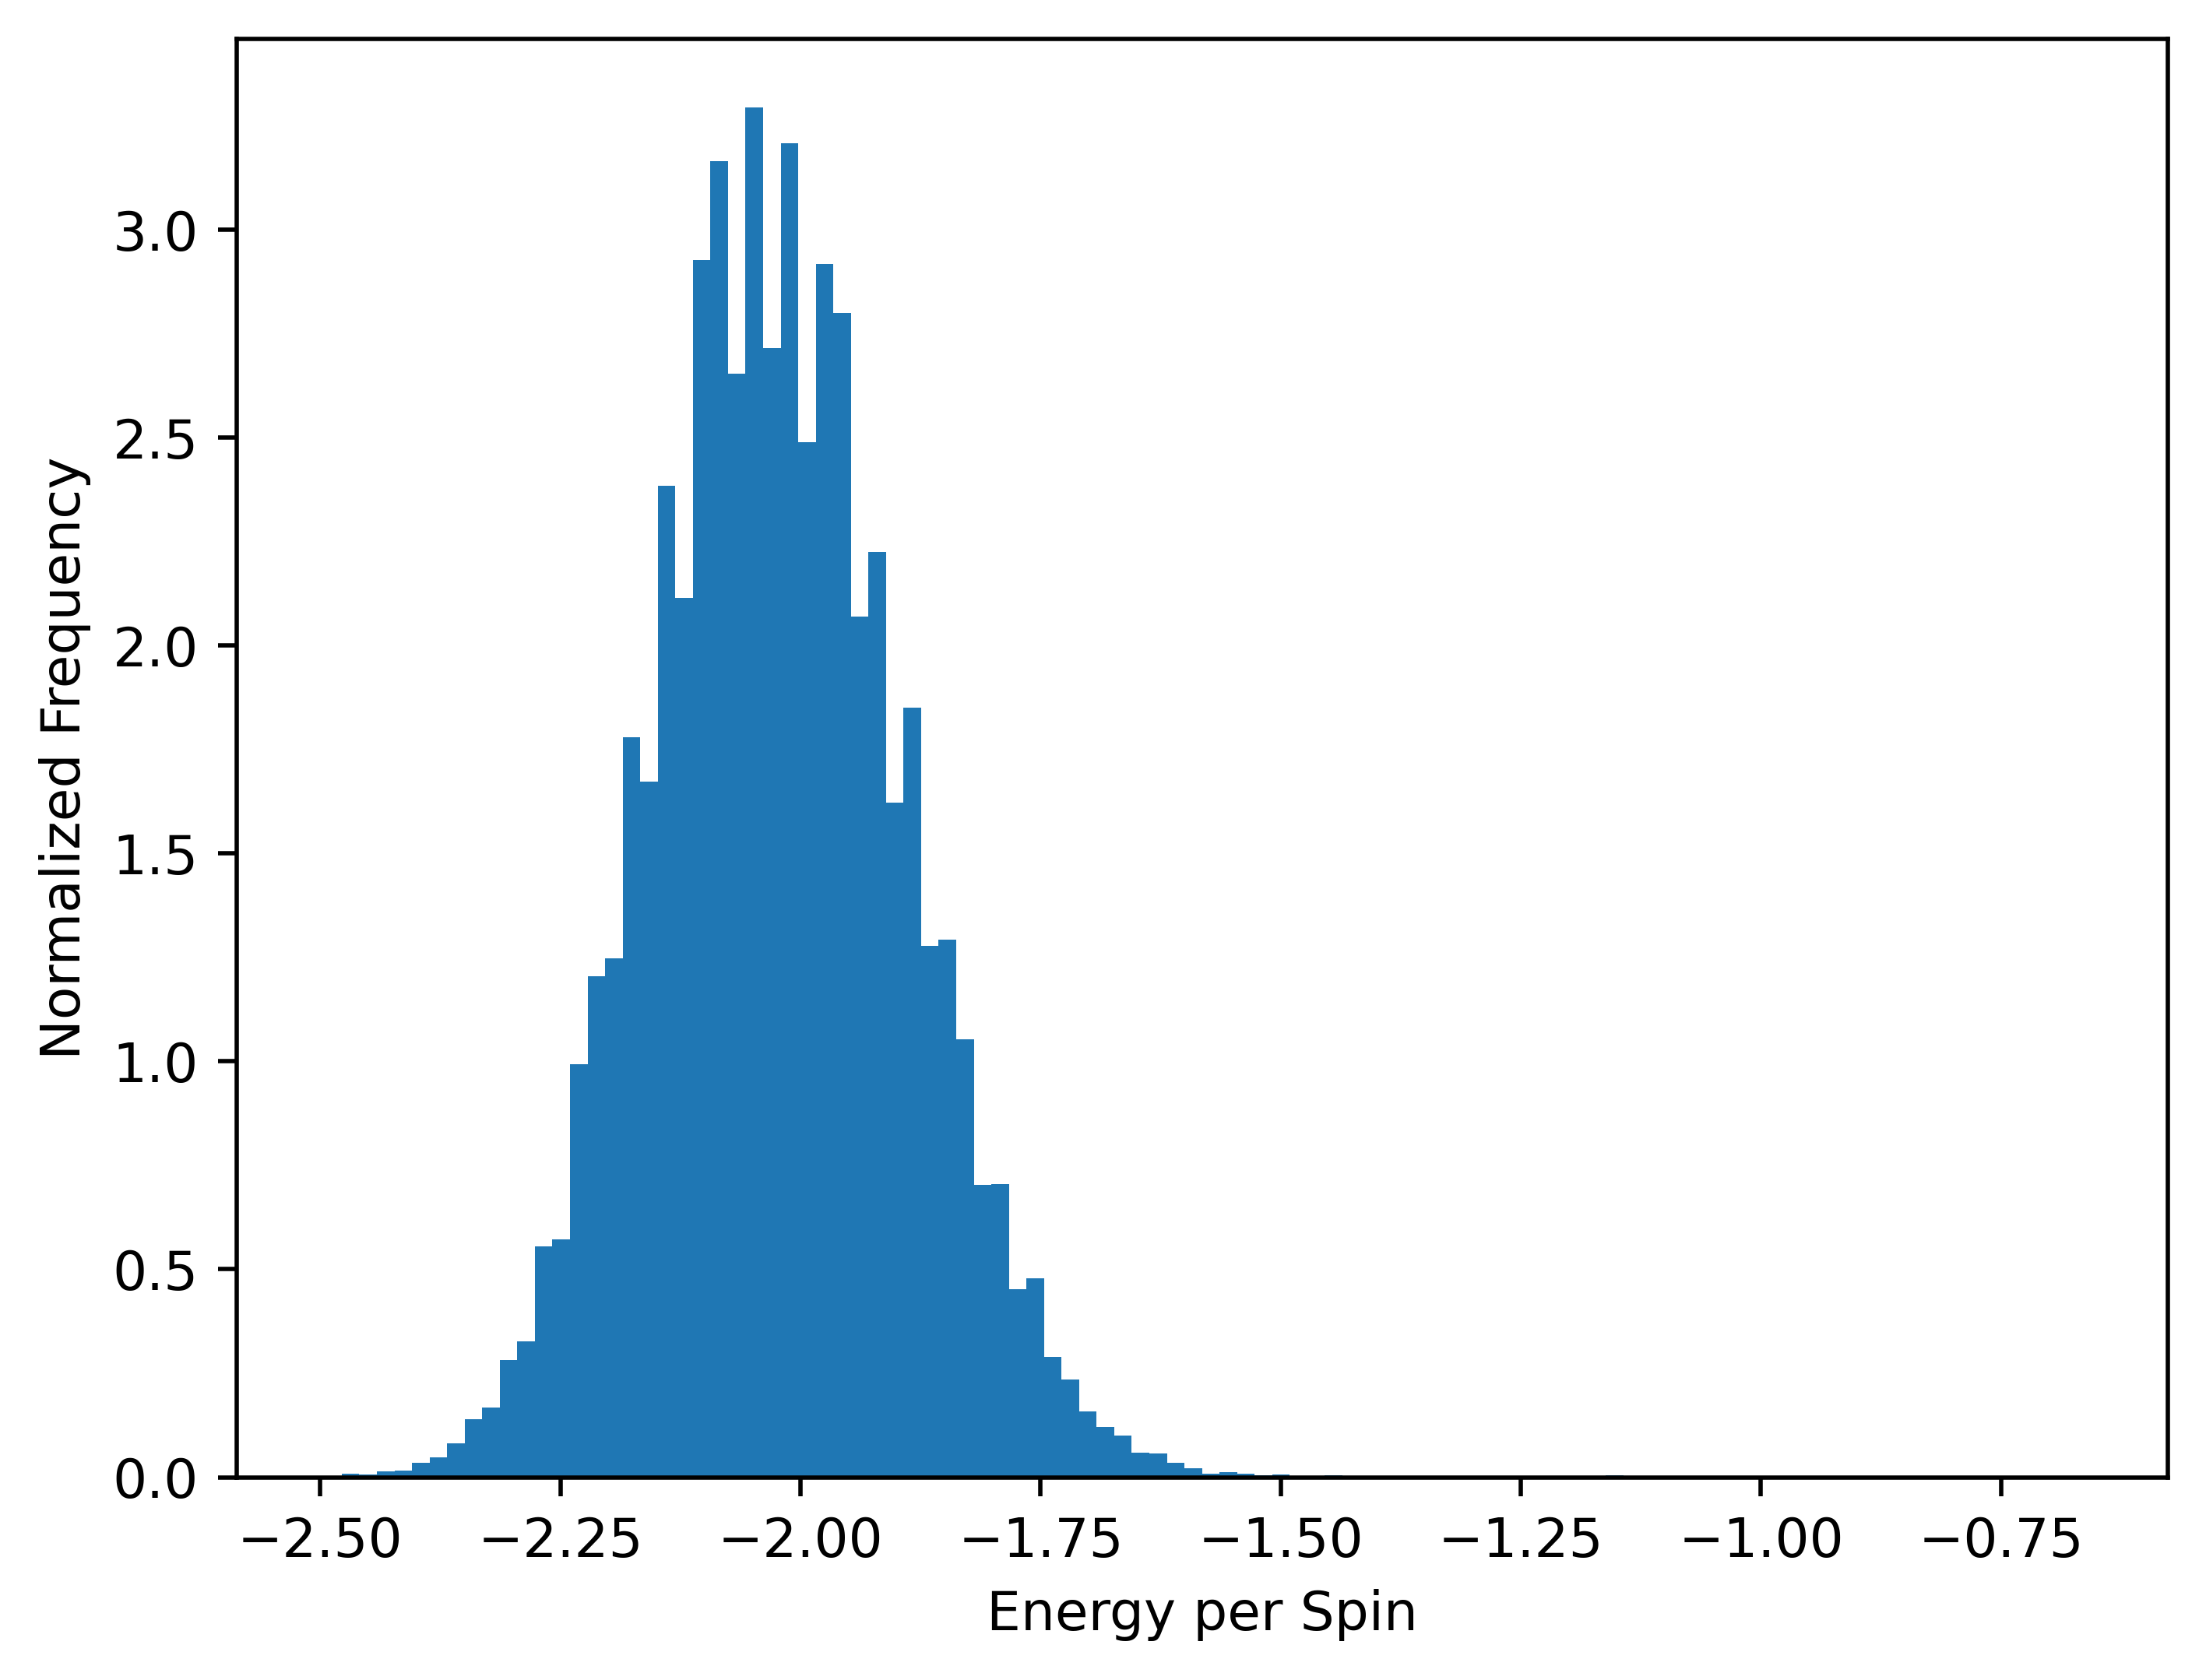
\includegraphics[scale=0.7]{4b.png}
\end{center}

\section*{5. a)}

We need to use brute force Monte Carlo in the interval $S^6$ where $S = [-a, a]$, let us get an estimate of the error of neglecting the region $\mathbb{R}^6 - S^6$.
\begin{align*}
    g(\vec{x}, \vec{y})                  & \leq \exp(-\vec{x}^2 - \vec{y}^2)                                                                           \\
    \implies \int_{\mathbb{R}^6 - S^6} g & \leq \int_{\mathbb{R}^6 - S^6} \exp(-\vec{x}^2 - \vec{y}^2) dx^3 dy^3                                       \\
                                         & = \int_{\mathbb{R}^6} \exp(-\vec{x}^2-\vec{y}^2)dx^3 dy^3 - \int_{S^6}  \exp(-\vec{x}^2-\vec{y}^2)dx^3 dy^3 \\
                                         & = \left(\int_{\mathbb{R}} \exp(-x^2) dx\right)^6 - \left(\int_S \exp(-x^2) dx\right)^6                      \\
\end{align*}
Let $m = \int_{S} \exp(-x^2) dx$, $n = \int_{\mathbb{R} - S} \exp(-x^2) dx$, then we can rewrite the above expression as
\begin{align*}
     & = (m + n)^6 - m^6                                               \\
     & = 6m^5 n + 15 m^4 n^2 + 20 m^3 n^3 + 15 m^2 n^4 + 6 m n^5 + n^6
\end{align*}
Clearly we are only concerned with the case where $n \ll m$, which simplifies things to
\begin{align*}
     & \leq 6m^5n + 57 m^4 n^2       \\
     & \leq 6(2a)^5n + 57 (2a)^4 n^2
\end{align*}
we can also write
\begin{align*}
    n = \sqrt{\pi} - \int_{-a}^{a} e^{-x^2} dx = \sqrt{\pi}\left(1 - \int_{-a\sqrt{2}}^{a\sqrt{2}} \mathcal{N}(x) dx \right)
\end{align*}
where $\mathcal{N}$ is the normal distribution.
For $a = 5$, $5\sqrt{2}$ corresponds to atleast $7\sigma$ deviations in the normal distribution which gives us
\begin{align*}
    n \leq \sqrt{\pi} (1 - 0.999999999997440) \approx 4.537 \cdot 10^{-12}
\end{align*}
Substituting back, we get
\begin{align*}
    \int_{\mathbb{R}^6 - S^6} g \leq 2.222 \times 10^{-6}
\end{align*}
which is a reasonable upper bound on the error.

Performing the integration with $N = 10^6$ (we keep this constant across all Monte Carlo integration methods), we get
\begin{align*}
    I \approx \input{../data/5a_val.dat}
\end{align*}
Error estimated by Monte Carlo is $\input{../data/5a_error_mc.dat}$ while actual error is $\input{../data/5a_error_actual.dat}$.

\section*{5. b)}

Now we do importance sampling with the Gaussian distribution in all 6 dimensions because the form of $g$ is similar to a Gaussian.
Performing the integration, we get
\begin{align*}
    I \approx \input{../data/5b_val.dat}
\end{align*}
Error estimated by Monte Carlo is $\input{../data/5b_error_mc.dat}$ while actual error is $\input{../data/5b_error_actual.dat}$.

We can also integrate using brute force in a finite region if we do the change of variables $x_i = \tan y_i$ in each dimension,
we get upon integration
\begin{align*}
    I \approx \input{../data/5c_val.dat}
\end{align*}
Error estimated by Monte Carlo is $\input{../data/5c_error_mc.dat}$ while actual error is $\input{../data/5c_error_actual.dat}$.

\end{document}
